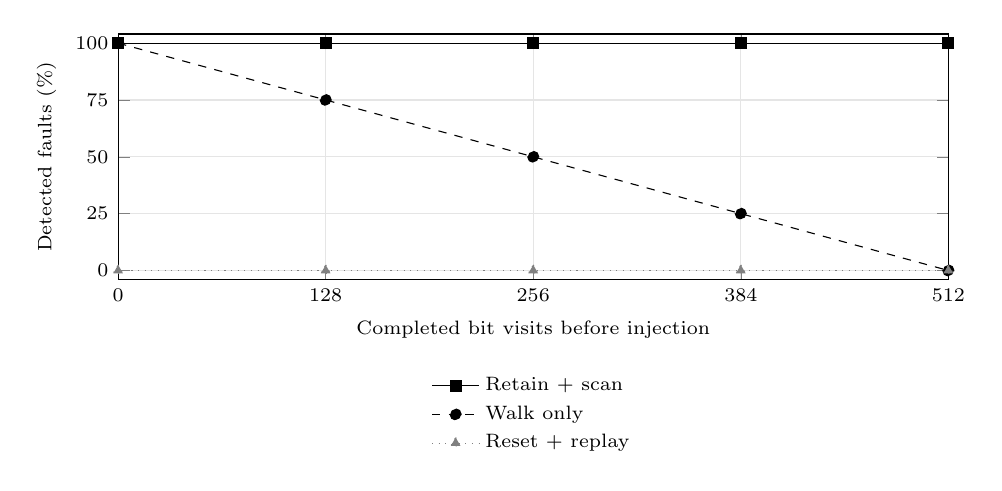
\begin{tikzpicture}
\begin{axis}[width=\columnwidth,height=4.7cm,
xlabel={Completed bit visits before injection},ylabel={Detected faults (\%)},
xmin=0,xmax=512,ymin=-4,ymax=104,xtick={0,128,256,384,512},ytick={0,25,50,75,100},
tick label style={font=\scriptsize},label style={font=\scriptsize},
legend style={font=\scriptsize,at={(0.5,-0.35)},anchor=north,draw=none},
grid=major,grid style={gray!20},legend cell align=left]
\addplot[black,mark=square*] coordinates {(0,100) (128,100) (256,100) (384,100) (512,100)};
\addlegendentry{Retain + scan}
\addplot[black,dashed,mark=*] coordinates {(0,100) (128,75) (256,50) (384,25) (512,0)};
\addlegendentry{Walk only}
\addplot[gray,dotted,mark=triangle*] coordinates {(0,0) (128,0) (256,0) (384,0) (512,0)};
\addlegendentry{Reset + replay}
\end{axis}
\end{tikzpicture}
